%
% $RCSfile: idea.tex,v $
%
% Copyright (C) 2002-2008. Christian Heller.
%
% Permission is granted to copy, distribute and/or modify this document
% under the terms of the GNU Free Documentation License, Version 1.1 or
% any later version published by the Free Software Foundation; with no
% Invariant Sections, with no Front-Cover Texts and with no Back-Cover
% Texts. A copy of the license is included in the section entitled
% "GNU Free Documentation License".
%
% http://www.cybop.net
% - Cybernetics Oriented Programming -
%
% http://www.resmedicinae.org
% - Information in Medicine -
%
% Version: $Revision: 1.1 $ $Date: 2008-08-19 20:41:07 $ $Author: christian $
% Authors: Christian Heller <christian.heller@tuxtax.de>
%

\section{Idea}
\label{idea_heading}

Researchers quite often follow the approach of first looking into what nature
offers and then trying to engineer a similar solution. All kinds of tools and
machines were created this way, even (and most obviously, with respect to the
human body and mind) robots and computers. Some scientists take the principles
of human awareness as physical model to explain the \emph{Universe} \cite{ripota}.
Some business people and consultants see analogies between processes in the
human brain and \emph{Organisational Structures of a Company} \cite{schoenhofer}.
Researchers in human sciences systematise \emph{International Public Law} by
sharing it into the three parts \emph{Society}, \emph{Cooperation} and
\emph{Conflicts} which are chosen in analogy to biology, that is \emph{Anatomy},
\emph{Physiology} and \emph{Pathology} of international relations \cite{bierzanek}.

Considering all that, one question is at hand: \textit{Why not apply a similar
approach to software engineering?} If computers are built after the model of
the human being (information input, memorising, processing and output), why not
structure the software that actually \emph{runs} those computers after similar
models? It seems logical and clear, yet the reality looks different. This work
wants to change that, and thereby help to improve application programming.

In search for new concepts to structure software, other sciences are called in.
The idea to marry systems sciences (notably general systems theory and cybernetics)
for analysis with creative problem solving techniques of designers for synthesis
is not new. Swift \cite{designmatrix} for example tried to apply both in form of
\emph{Cyberpatterns} to complex systems problems, using a pattern language. Yet
while Swift had turned his attention to what he calls \textit{the extreme front
end}, this work goes one step further. It applies the principles of nature
(results of many different sciences) not only to the \emph{User Interface}
(frontend) of an application, but to whole software system architectures.

\begin{figure}[ht]
    \begin{center}
        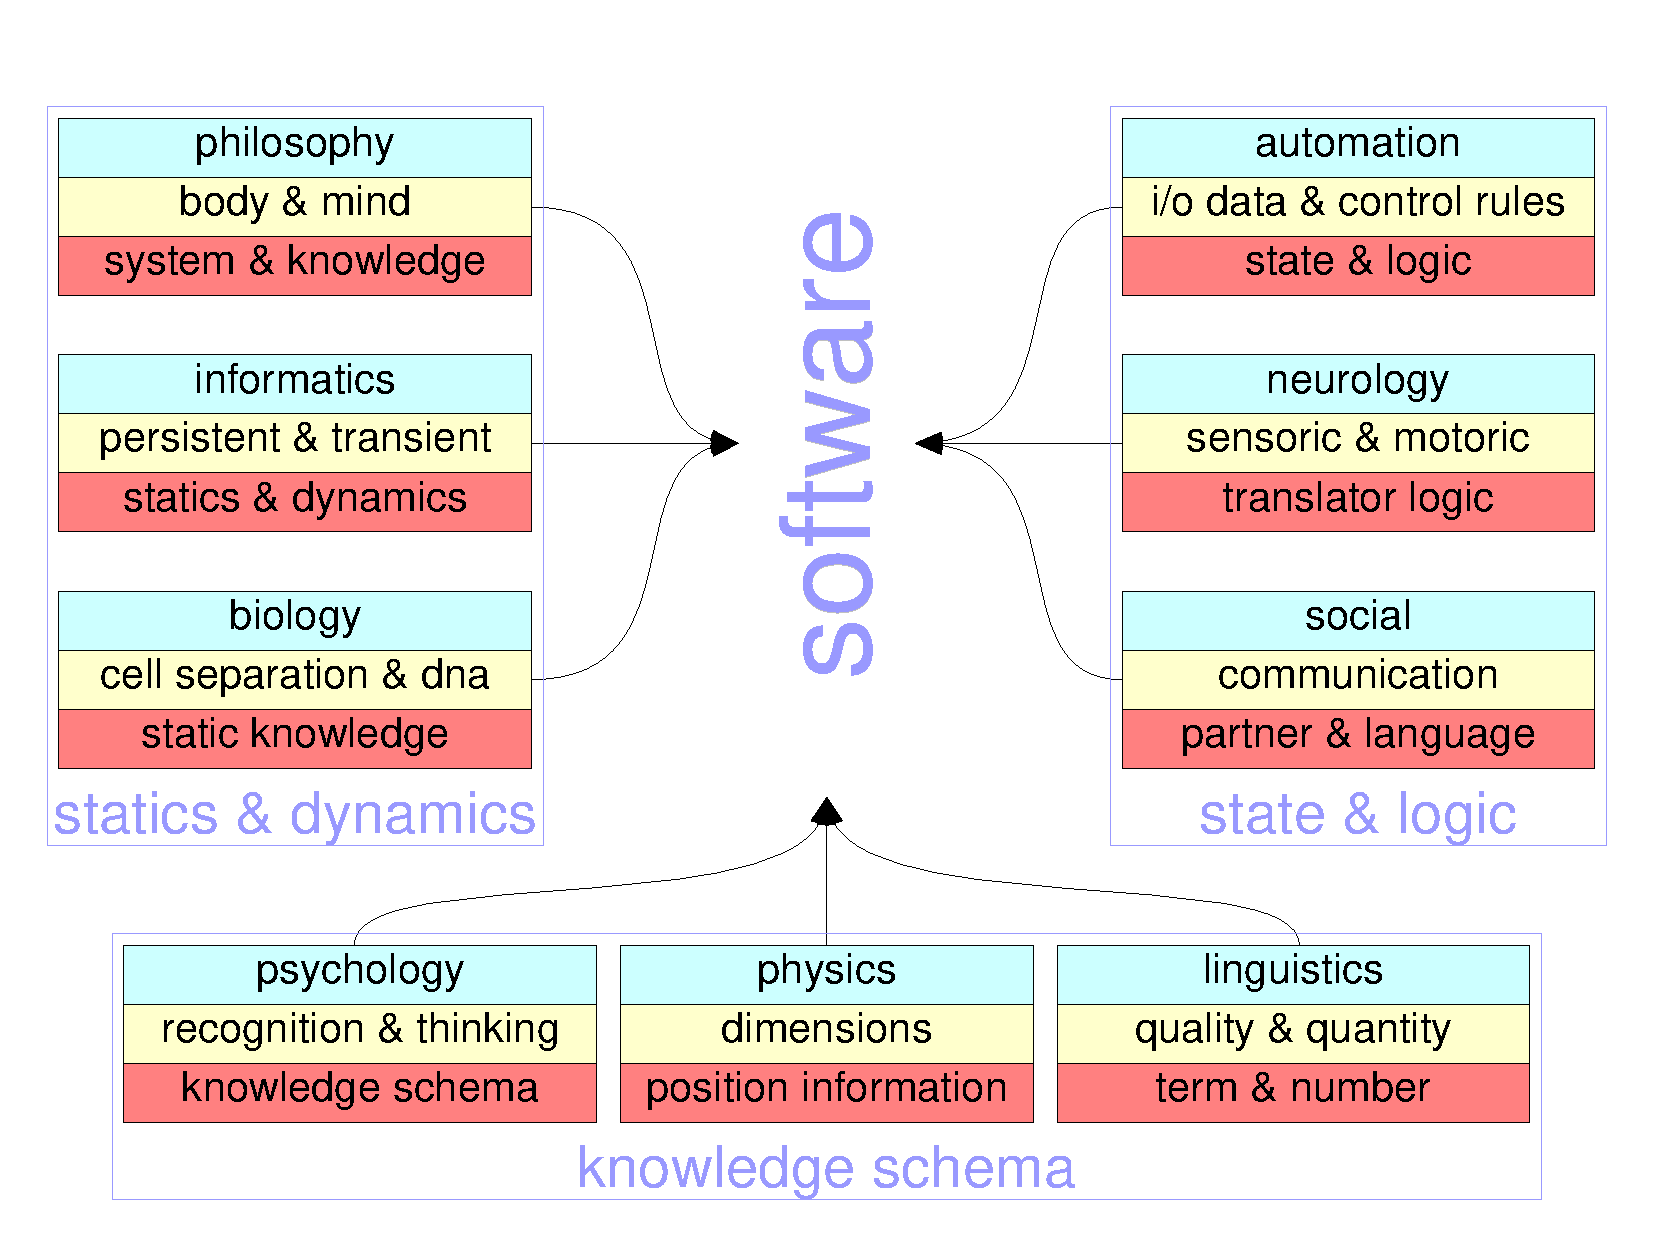
\includegraphics[scale=0.3,angle=-90]{graphic/mindmap.pdf}
        \caption{Mindmap of Sciences whose Principles influenced CYBOP}
        \label{mindmap_figure}
    \end{center}
\end{figure}

Figure \ref{mindmap_figure} shows some of the sciences whose principles were
considered in this work. The name of a field of science is shown on top of each
box. Made observations are mentioned below, in the middle. The resulting design
recommendations for software can be found at the bottom of each box. The
recommendations are grouped into those that justify a separation of
\emph{Statics and Dynamics} (left-hand side), a new kind of
\emph{Knowledge Schema} (lower part of the figure) and a distinction between
\emph{State and Logic} models (right-hand side).

It has to be mentioned though, that only some of the principles underlying a
specific field of science were considered in the figure and in more detail
later in this work. The figure does by no means claim to be complete. The shown
observations are only those that seemed promising in the context of software
design. The existence of persistent and transient data, for example, is only
one of many aspects of the science of informatics. Similarly is the existence
of sensoric and motoric nerve system just one aspect of the field of neurology.
And so on. Further details on the mentioned sciences and observations are not
given here, since later chapters will elaborate on them.
